%----------------------------------------------------------------------------------------
%	PACKAGES AND OTHER DOCUMENT CONFIGURATIONS
%----------------------------------------------------------------------------------------

\documentclass[9pt]{developercv}
\usepackage{graphicx}
\usepackage[export]{adjustbox}
%----------------------------------------------------------------------------------------

\begin{document}

%----------------------------------------------------------------------------------------
%	TITLE AND CONTACT INFORMATION
%----------------------------------------------------------------------------------------

\begin{minipage}[t]{0.3\textwidth}
	\vspace{-\baselineskip}
	\colorbox{black}{{\Huge\textcolor{white}{\textbf{\MakeUppercase{Ionut Daniel}}}}}
	
	\colorbox{black}{{\Huge\textcolor{white}{\textbf{\MakeUppercase{Fagadau}}}}}
	
	\vspace{6pt}
	
	{\Large 17 Gennaio 1999 \\ Dorohoi, Romania}
\end{minipage}
\begin{minipage}[t]{0.22\textwidth} % 27.5% of the page width for the first row of icons
	\vspace{-\baselineskip} % Required for vertically aligning minipages
	
	% The first parameter is the FontAwesome icon name, the second is the box size and the third is the text
	% Other icons can be found by referring to fontawesome.pdf (supplied with the template) and using the word after \fa in the command for the icon you want
	\icon{MapMarker}{12}{Novara}\\
	
	\icon{Github}{12}{\href{https://github.com/Mooyeee}{Daniel Fagadau}}\\
\end{minipage}
\begin{minipage}[t]{0.3\textwidth}
\vspace{-\baselineskip}
\icon{At}{12}{danielfagadau@gmail.com}\\

	\icon{Linkedin}{12}{\href{https://www.linkedin.com/in/daniel-fagadau/}{daniel-fagadau}} \\	
\end{minipage}
\begin{minipage}[t]{0.2\textwidth}
\vspace{-\baselineskip}
\noindent
\centering
\vspace{-20mm}{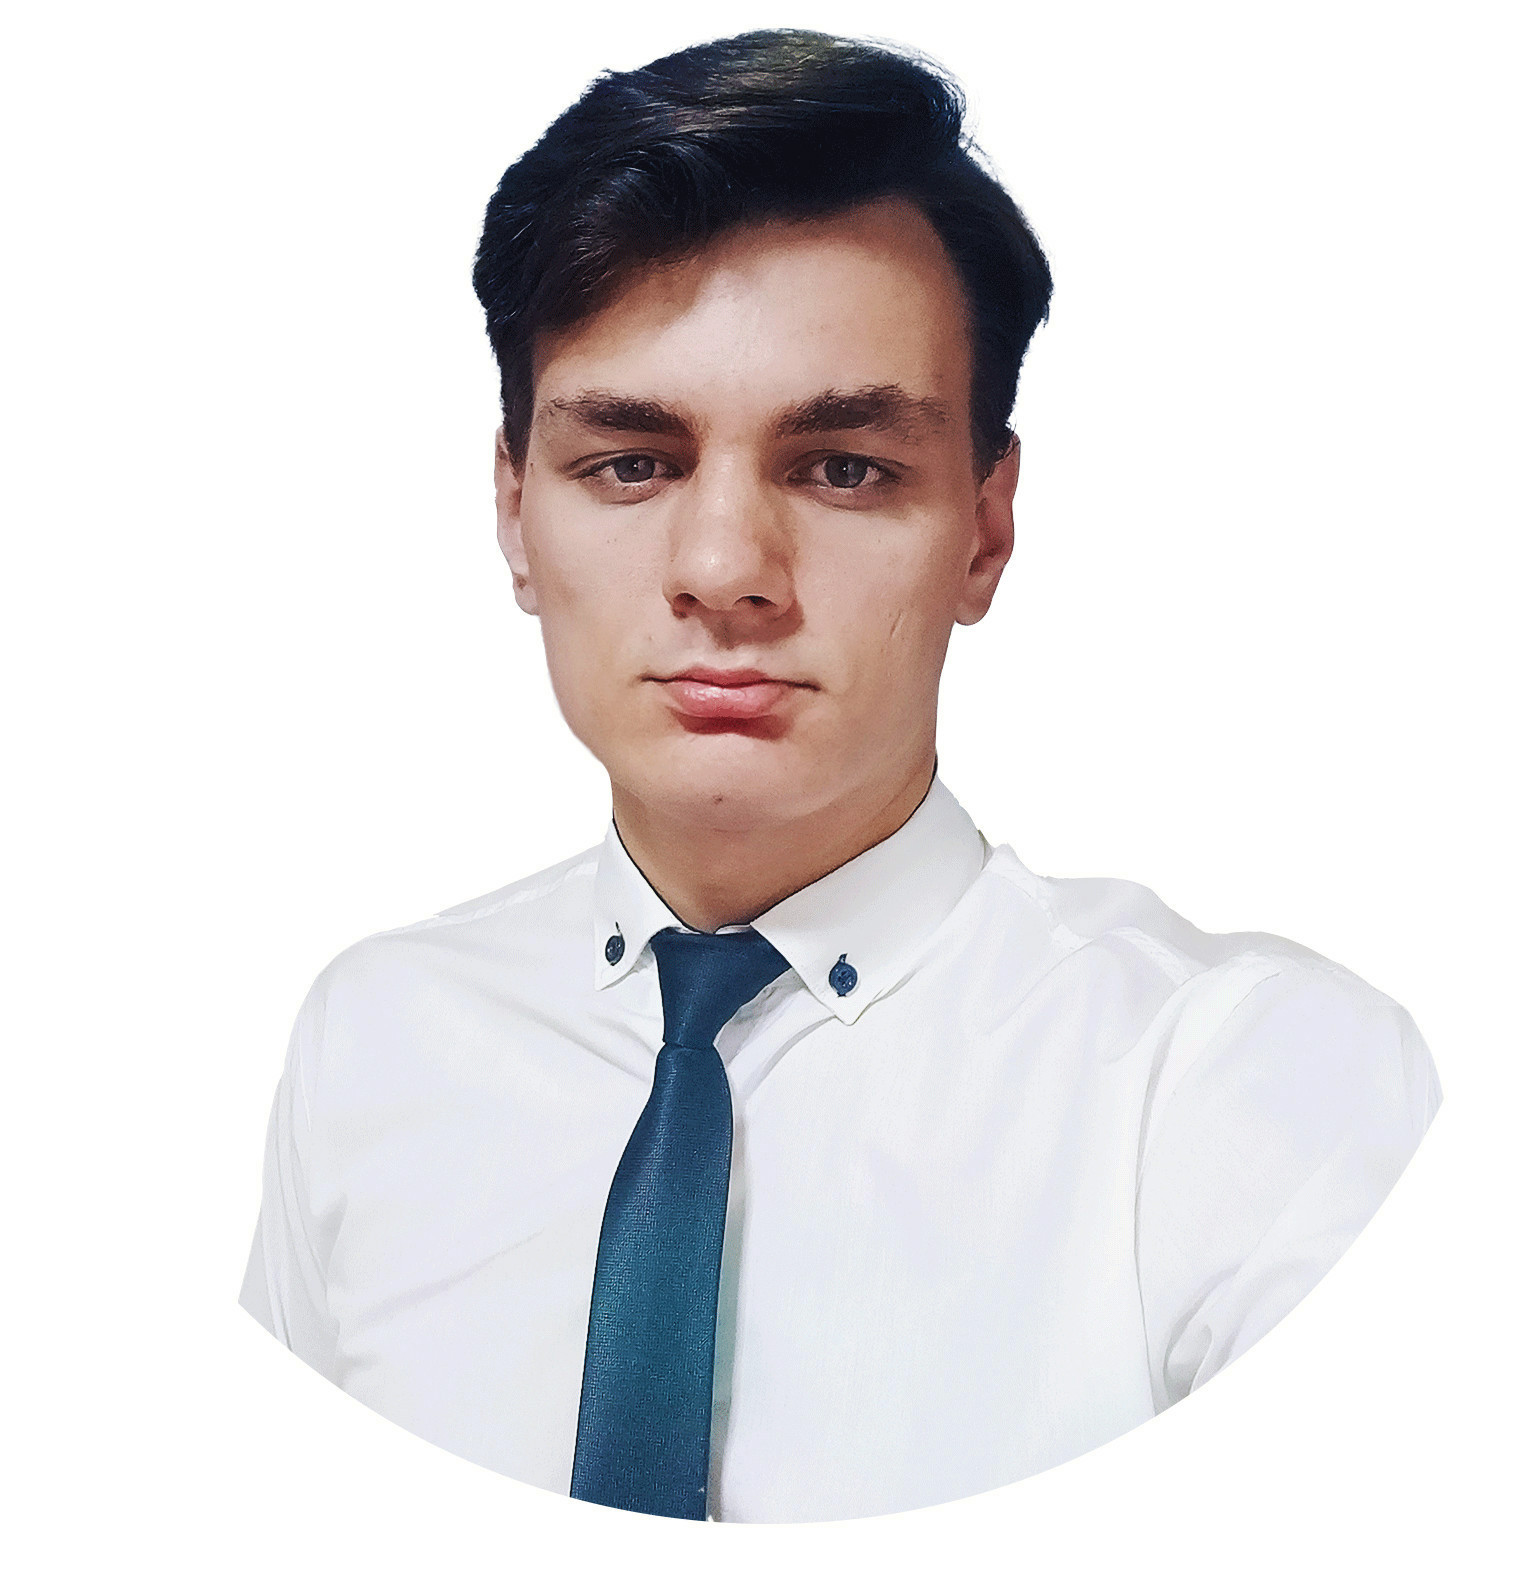
\includegraphics[scale=0.045, center]{foto_cv}}
\end{minipage}

\vspace{0.5cm}


%----------------------------------------------------------------------------------------
%	EXPERIENCE
%----------------------------------------------------------------------------------------

\cvsect{Esperienza professionale}

\begin{entrylist}
	\entry
	{15/03/2022 \\ 17/05/2022}
	{Esercitatore di Algoritmi e Programmazione [E3501Q067]}
	{Università degli Studi di Milano - Bicocca}
	{Svolgimento esercitazioni frontali in laboratorio per il corso di Algoritmi e Programmazione del secondo anno del corso di Laurea Triennale in Matematica.}

	\entry
	{Settembre 2021 \\ Settembre 2022	\\\footnotesize{smart working}}
	{Borsa di Ricerca - Proactive Modules}
	{Università degli Studi di Milano - Bicocca}
	{Attività di ricerca su tecniche di self-repair in Android sfruttando il framework Xposed per rilevare e risolvere a runtime violazioni di policy riguardanti l'utilizzo delle API Android. Sviluppo di tool Eclipse che permeta la generazione di librerie proattive a partire da automi a stati finiti. \\ \texttt{Java}\slashsep\texttt{Eclipse PDE, EMF \& GMF}\slashsep\texttt{Acceleo}\slashsep\texttt{Apache Maven}\slashsep\texttt{Gradle}\slashsep\texttt{Flutter}}
	
	\entry
		{Marzo 2020 \\ Presente \\\footnotesize{smart working}}
		{MindBlooming: una soluzione mobile a supporto della CBT}
		{Università degli Studi di Milano - Bicocca}
		{Continuazione del lavoro iniziato durante lo stage assieme alla prof.ssa Daniela Micucci e al dott. Davide Ginelli in collaborazione col dipartimento di Psicologia UniMiB. \\ \texttt{Java}\slashsep\texttt{Dart}\slashsep\texttt{Flutter}}
	\entry
		{Dicembre 2020 \\ Marzo 2020\\\footnotesize{smart working}}
		{Stage sviluppo cross-platform con Flutter}
		{Università degli Studi di Milano - Bicocca}
		{Applicazione multi-piattaforma a sostegno della terapia cognitivo comportamentale. Acquisite ottime conoscenze dell'ambiente mobile e del framework Flutter. Sviluppate anche problem solving, lavoro autonomo, self-learning, lavoro per obiettivi, pianificazione e organizzazione. \\ \texttt{Java}\slashsep\texttt{Dart}\slashsep\texttt{Flutter}}
	\entry
		{3/9/2018  21/9/2018}
		{Elmec SmartCollege}
		{Elmec Informatica S.P.A. - Varese}
		{Corso intensivo di formazione su web design, sviluppo web e cross-platform, UI e UX Design. \\ \texttt{node.js}\slashsep\texttt{Vue.js}\slashsep\texttt{React Native}}
	\entry
		{2016 -- 2018\\\footnotesize{part time}}
		{Grafica Sito web \& Gestione database}
		{Indieversus - Novara}
		{Grafica pubblicitaria e sviluppo e mantenimento di sito web. Sviluppata buona gestione del tempo. \\ \texttt{HTML}\slashsep\texttt{PHP}\slashsep\texttt{JavaScript}\slashsep\texttt{Adobe Photoshop}\slashsep\texttt{Adobe After Effects}}
	\entry
		{2016 -- 2018}
		{Alternanza Scuola Lavoro}
		{ITIS G. Fauser - Novara}
		{Esercitazioni CISCO, esperienze di laboratorio ed incontri informativi su Industria 4.0 \& IoT. \\ \texttt{C}\slashsep\texttt{C\#}\slashsep\texttt{C++}\slashsep\texttt{Cisco Packet Tracer}}
\end{entrylist}

%----------------------------------------------------------------------------------------
%	EDUCATION
%----------------------------------------------------------------------------------------

\cvsect{Istruzione e formazione}

\begin{entrylist}
	\entry
		{2021 -- presente}
		{Laurea Magistrale - Informatica}
		{Università Degli Studi di Milano Bicocca}
		{Media Ponderata attuale: 29.333}
	\entry
		{2018 -- 2021}
		{Laurea Triennale - Informatica}
		{Università Degli Studi di Milano Bicocca}
		{Conseguimento laurea triennale in Informatica con voto 110L/110.}
	\entry
		{2015 -- 2018}
		{Diploma esame di stato - profilo informatico}
		{ITIS G. Fauser - Novara}
		{Voto: cento/centesimi}
	\entry
		{2013 -- 2015}
		{Biennio profilo informatico}
		{ITIS H. Hertz - Roma}
		{Ho svolto i primi due anni di liceo a Roma.}
\end{entrylist}

%----------------------------------------------------------------------------------------
%	ADDITIONAL INFORMATION
%----------------------------------------------------------------------------------------

\begin{minipage}[t]{0.3\textwidth}
	\vspace{-\baselineskip}

	\cvsect{Lingue}
	
	\textbf{Inglese} - C1 certificato CAE\\
	\textbf{Italiano} - Lingua madre\\
	\textbf{Rumeno} - Lingua madre
\end{minipage}
\hfill
\begin{minipage}[t]{0.3\textwidth}
	\vspace{-\baselineskip}
	
	\cvsect{Borse di Studio}
	
	\textbf{TalentAward} - Elmec, 2018 \\
	\textbf{Giuseppe Sironi} - G. Fauser, 2017 \\
	\textbf{Borsa di ricerca} - UniMiB, 2021
\end{minipage}
\hfill
\begin{minipage}[t]{0.3\textwidth}
	\vspace{-\baselineskip}
	
	\cvsect{Patente di guida}
	
	B
\end{minipage}

%----------------------------------------------------------------------------------------

\vskip 0.8em
\cvsect{Dati Personali}

Autorizzo il trattamento dei miei dati personali ai sensi del Decreto Legislativo 30 giugno 2003, n. 196 "Codice in materia di protezione dei dati personali”.

\end{document}
